% !TEX root = main.tex

\section{Figures}

We parse the optional argument to \texttt{includegraphics}. The \texttt{Image} class has an attribute \texttt{width} expressed as a percentage. This is computed from the (optional) \texttt{scale} or \texttt{width} parameters passed to \texttt{includegraphics}.

\begin{itemize}
\item \autoref{fig:acapb} is a nice size (scale = 0.25).
\item \autoref{fig:acapb-big} is a bigger version (scale = 0.5).
\item \autoref{fig:setops-tabular} shows a figure layout using \texttt{tabular}. %The optional parameter to \texttt{includegraphics} is \texttt{scale=0.4}, and the pictures take up 40\% of each cell, which is a pity.
\end{itemize}

% basic
Here is a figure with {\tt scale=0.25}:
\begin{figure}[ht]
\centering
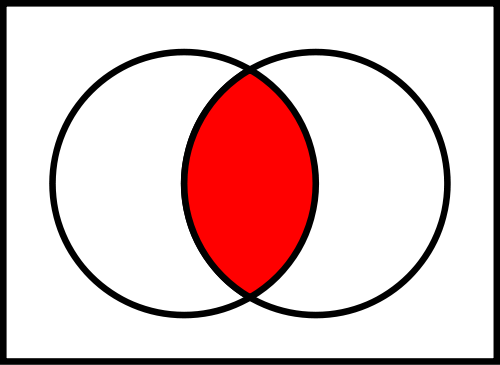
\includegraphics[scale=0.25]{AcapB}
\caption{Set intersection (scale=0.25)\label{fig:acapb}}
\end{figure}

% big
Here is the same figure with {\tt scale=0.5}:
\begin{figure}[ht]
\centering
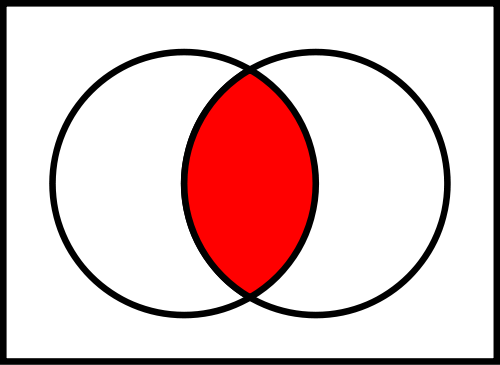
\includegraphics[scale=0.5]{AcapB}
\caption{A bigger version\label{fig:acapb-big}}
\end{figure}

Here are nested {\tt minipages} with {\tt scale=0.4}:
\begin{framed}
\begin{minipage}{\textwidth}
\begin{minipage}{0.5\textwidth}
\lipsum[2-2]
\end{minipage}
\begin{minipage}{0.5\linewidth}
\quad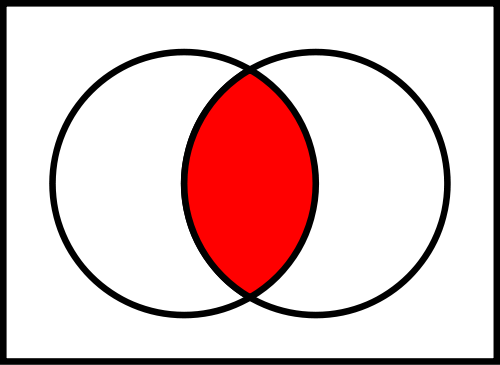
\includegraphics[scale=0.4]{AcapB}
\end{minipage}
\end{minipage}
\end{framed}

Here are nested {\tt minipages} with {\tt width=0.8*linewidth}:
\begin{framed}
\begin{minipage}{\textwidth}
\begin{minipage}{0.5\textwidth}
\lipsum[2-2]
\end{minipage}
\begin{minipage}{0.5\linewidth}
\qquad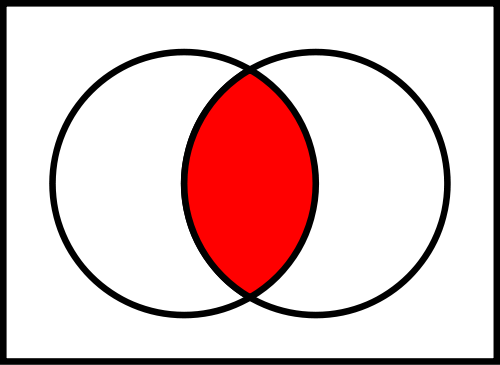
\includegraphics[width=0.8\linewidth]{AcapB}
\end{minipage}
\end{minipage}
\end{framed}

% three in a row
%\begin{tabular}{ccc}
%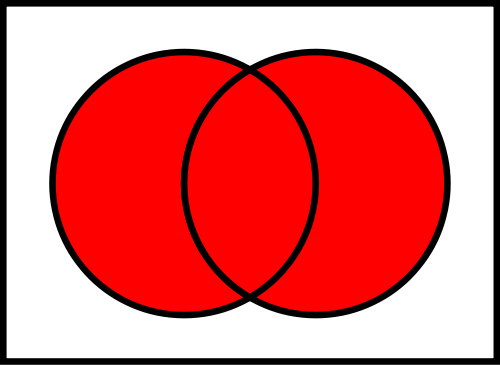
\includegraphics[width=\linewidth]{AcupB}
%&
%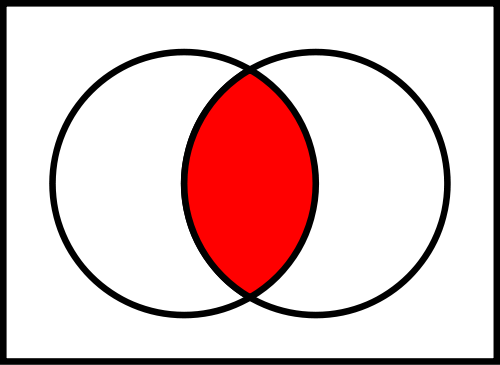
\includegraphics[width=\textwidth]{AcapB}
%&
%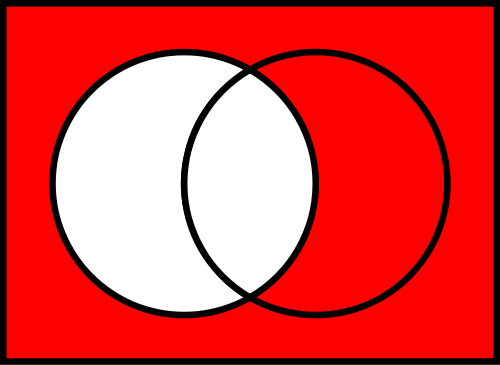
\includegraphics[width=\textwidth]{Acomp}
%\\
%Union & Intersection & Complementation
%\\
%\end{tabular}

Here are three images in a {\tt tabular} inside a {\tt figure}:
% float
\begin{figure}[ht]
\centering
\begin{tabular}{ccc}
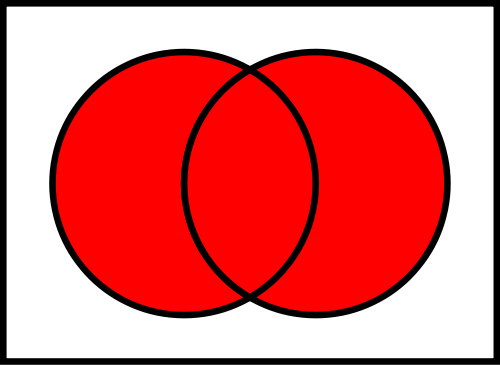
\includegraphics[scale=0.25]{AcupB}
&
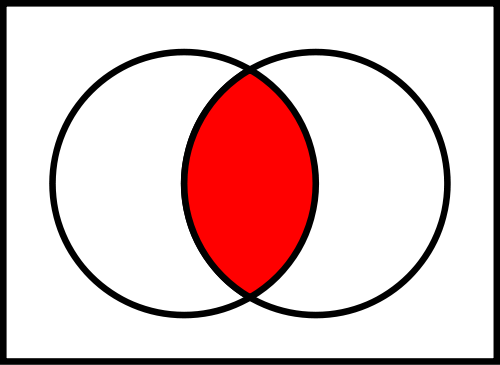
\includegraphics[scale=0.25]{AcapB}
&
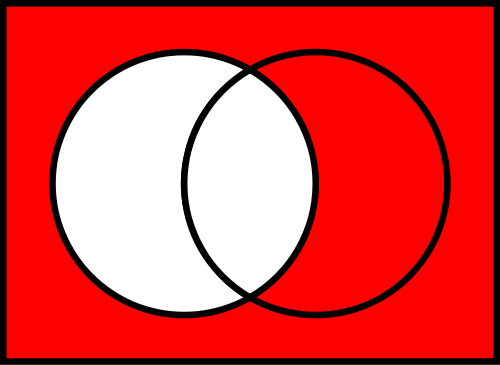
\includegraphics[scale=0.25]{Acomp}
\\
Union & Intersection & Complementation
\\
\end{tabular}
\caption{Three images in a {\tt tabular} inside a \texttt{figure}.\label{fig:setops-tabular}}
\end{figure}

%\begin{figure}
%\centering
%\begin{tabular}{ccc}
%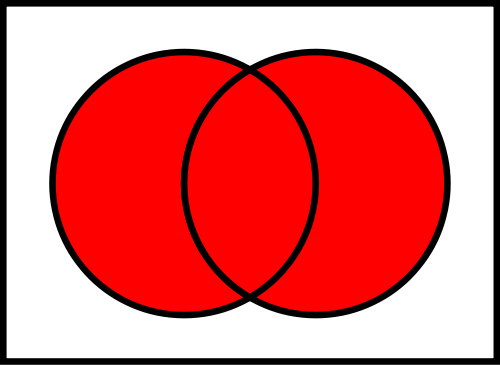
\includegraphics[width=0.25\linewidth]{AcupB} &
%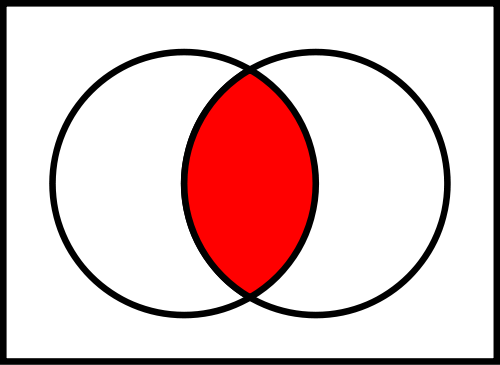
\includegraphics[width=0.25\textwidth]{AcapB} &
%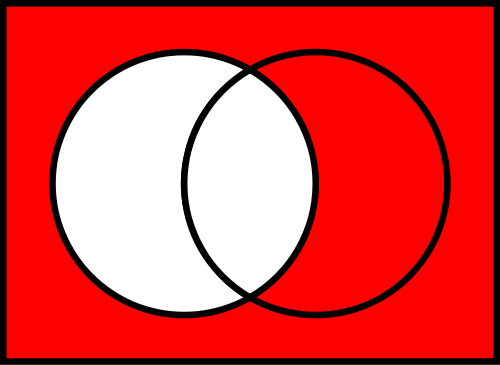
\includegraphics[width=0.25\textwidth]{Acomp} \\
%(a) Union & (b) Intersection & (c) Complementation \\
%\end{tabular}
%\caption{Three figures using \texttt{tabular}.\label{fig:setops-tabular}}
%\end{figure}
